\section{Δημιουργία αμφιωτικών σημάτων} \label{sec:bin_sig_creation}

\noindent
Τα σήματα που περιγράφονται στην υποενότητα \ref{sec:input_signals} στη συνέχεια συνελίσονται με BRIRs, για διαφορετικές γωνίες, που προέρχονται από τρία δωμάτια: Το TU Berlin Auditorium 3 \cite{Wierstorf2016b}, το Spirit \cite{Wierstorf2016a}, και το Calypso \cite{Wierstorf2016}. Σε κάθε περίπτωση, το ανδρείκελο απείχε 1m από την πηγή, ενώ έγιναν μετρήσεις με ανάλυση $1^o$ στο οριζόντιο επίπεδο, από $-90^o$ μέχρι $+90^o$ χρησιμοποιώντας το ανδρείκελο KEMAR και ηχεία Genelec, τοποθετημένα σε ανύψωση $0^o$. 

Στην εργασία αυτή χρησιμοποιήθηκε ανάλυση στο οριζόντιο επίπεδο $2^o$, με αποτέλεσμα να προκύψουν 91 κρουστικές για κάθε δωμάτιο. Χρησιμοποιήθηκαν και τα τρία δωμάτια, και άρα μετά από τη συνέλιξη κάθε ενός από τα 29 σήματα εισόδου, με μία από τις $3 * 91 = 273$ διαφορετικές κρουστικές, δημιουργούνται συνολικά $29 * 273 = 7917$ διαφορετικά σήματα εισόδου.

Αναλυτικότερα, αφού φορτωθεί το εκάστοτε dataset, και από αυτό διαβαστεί η BRIR, η οποία εμφανώς αποτελείται από δύο κανάλια διότι είναι binaural, εφαρμόζεται σε αυτή ένα παράθυρο Half Hanning μήκους 9000 δειγμάτων, αφού ρυθμιστεί η ζητούμενη δειγματοληψία. Τα δύο κανάλια της BRIR συνελίσονται με το mono σήμα εισόδου και προκύπτει το αμφιωτικό σήμα από το οποίο θα εξαχθούν στη συνέχεια οι αμφιωτικές παράμετροι. Έτσι, το αποτέλεσμα της συνέλιξης είναι ένα αμφιωτικό σήμα διαστάσεων $[2,L]$, όπου $L = M + N - 1 = 17819$, με δεδομένο ότι η BRIR έχει μήκος $M = 9000$ δείγματα και το mono σήμα μήκος $N = 8820$ δείγματα.

Η παραθύρωση έγινε λόγω περιορισμών στους υπολογιστικούς πόρους, αλλά επιλέχθηκε τέτοιο μέγεθος παραθύρου ώστε να διατηρούνται τα σημαντικότερα χαρακτηριστικά των BRIR. 

Μια κρουστική μαζί με το παράθυρο που εφαρμόζεται σε αυτή και η BRIR μετά την εφαρμογή του, φαίνονται στο Σχήμα \ref{fig:brir_processing}. Συνοπτικά η διαδικασία της δημιουργίας των αμφιωτικών σημάτων φαίνεται στο Σχήμα \ref{fig:binaural_signal_gen_block}.

\begin{figure}[h]
  \centering
  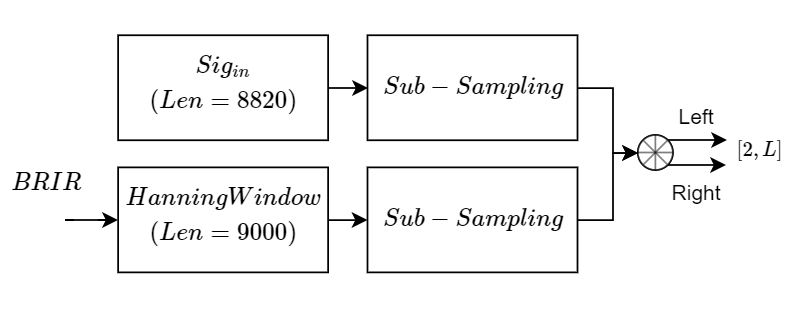
\includegraphics[width=\textwidth]{images/binaural_signal_gen_block.png}
  \caption{Δημιουργία αμφιωτικών σημάτων. Το block sub-sampling χρησιμοποιείται μόνο στην περίπτωση που τα σήματα έχουν διαφορετική δειγματοληψία από την επιθυμητή $f_s = 44.1 kHz$}
  \label{fig:binaural_signal_gen_block}
\end{figure}

\begin{figure}
     \centering
     \begin{subfigure}[b]{\textwidth}
         \centering
         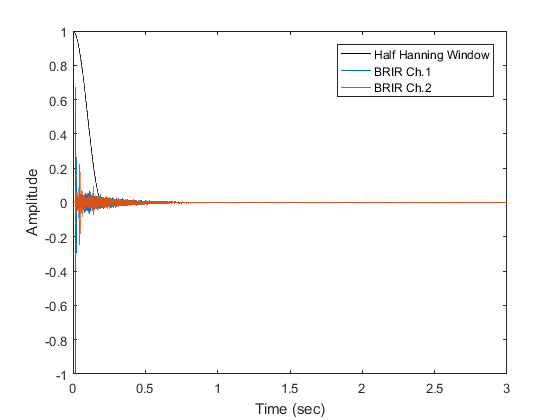
\includegraphics[width=\textwidth]{images/brir_window.png}
         \caption{}
         \label{fig:brir_window}
     \end{subfigure}
     \hfill
     \begin{subfigure}[b]{\textwidth}
         \centering
         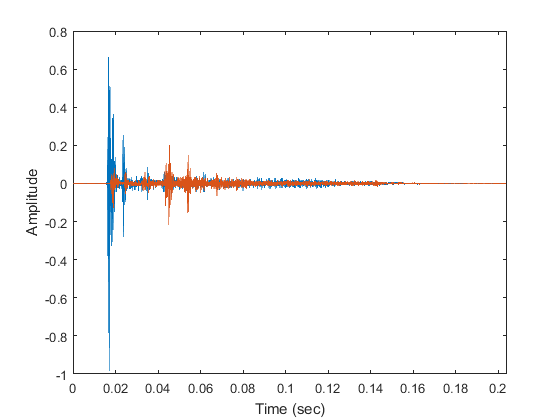
\includegraphics[width=\textwidth]{images/windowed_brir.png}
         \caption{}
         \label{fig:windowed_brir}
     \end{subfigure}
        \caption{(α'): BRIR και το αντίστοιχο Half Hanning παράθυρο, (β'): BRIR μετά την παραθύρωση. Τα σχήματα είναι για $f_s = 44.1 kHz$ }
        \label{fig:brir_processing}
\end{figure}